\chapter{\mFourL: A measurement designed for re-interpretation}
\label{chap:fourlepton}

\chapterquote{Very inspiring quote}
{Very inspiring quote author}

%% m4l motivation
\section{Motivation for the \mFourL measurement}
\label{sec:fourlepmotivation}

The four lepton channel is a particularly interesting channel to study as it receives contributions from many physics processes.  

First and foremost, there is the production of a pair of \PZ-bosons via quark-antiquark interactions in \info[]{s-channel not in SM because it includes neutral ZZZ or ZZ\photon vertex} both the \Ptop- and \Pup-channel. The \Ptop-channel diagram is shown in Figure \ref{fig:m4lfeynman:qqZZ}, and represents, by far, \improvement[]{Read more about why the u-channel diagram is not preferred} the largest contribution to the \ZZ production and thus to the \mFourL distribution. At the low mass end where $\mFourL=m_{PZ}$, there is resonant production of a single \PZ boson via the s-channel diagram in Figure \ref{fig:m4lfeynman:singleZ}. At $\mFourL=\unit{180}{\GeV}$ and beyond, the threshold for the on-shell production of two \PZ bosons is reached and results in a peak in the four lepton invariant mass spectrum. 

Second in magnitude is the gluon-induced production of a \PZ boson pair. This occurs via a triangle or box quark loop, which results in a factor $\alpha_s^2$ suppression. It still plays a substantial role, however, because at small $x$\footnote{Here $x$ is the component of the proton's momentum carried by the struck quark. At the \LHC the protons have very high energies; therefore the \LHC can be described as a small $x$ collider \cite{zotov2012small}} gluon-gluon luminosity is higher than the quark-antiquark luminosity \cite{Glover:194539}. The contribution from this process in on the order of ten percent \cite{Becker:2230817}. Finally in the pool of \PZ boson pairs there is a small contribution from decaying Higgs bosons, which themselves are produced also via gluon fusion, as illustrated in Figure \ref{fig:m4lfeynman:ggHZZ}. There is resonant Higgs production at \mFourL=\unit{125}{\GeV}, and a non-resonant enhancement at $\mFourL=m_{\Ptop}=\unit{350}{\GeV}$ from the top quark loop. Beyond \unit{350}{\GeV}, the Higgs-mediated \PZ boson pair production process destructively interferes with continuum production of on-shell \PZ bosons \cite{Campbell_2016}.

The \mFourL distribution can be a useful probe for certain new physics scenarios. Take for example, the high mass tail of the invariant mass spectrum. This region is dependent on the couplings of the Higgs to incoming and outgoing particles while independent of the Higgs boson width \cite{Campbell_2016}, a unique property that can be exploited to derive model-independent limits on the Higgs couplings, and on the \todo{reword, this is copy pasted} contribution of new states in the Higgs to gluon coupling \cite{Cacciapaglia_2014}. It has also been previously exploited to derive model-independent constraints on the Higgs boson width \cite{Caola_2013}. 

%% Secondly, under specific assumptions a class of models exists for which the off-shell coupling measurement together with a measurement of the on-shell signal strength can be re-interpreted in terms of a bound on the total Higgs boson width. In this paper, we provide a first step towards a classification of the models for which a total width measurement is viable and we discuss examples of BSM models for which the off-shell coupling measurement can be important in either constraining or even discovering new physics in the upcoming LHC runs

\begin{figure}
    \centering
    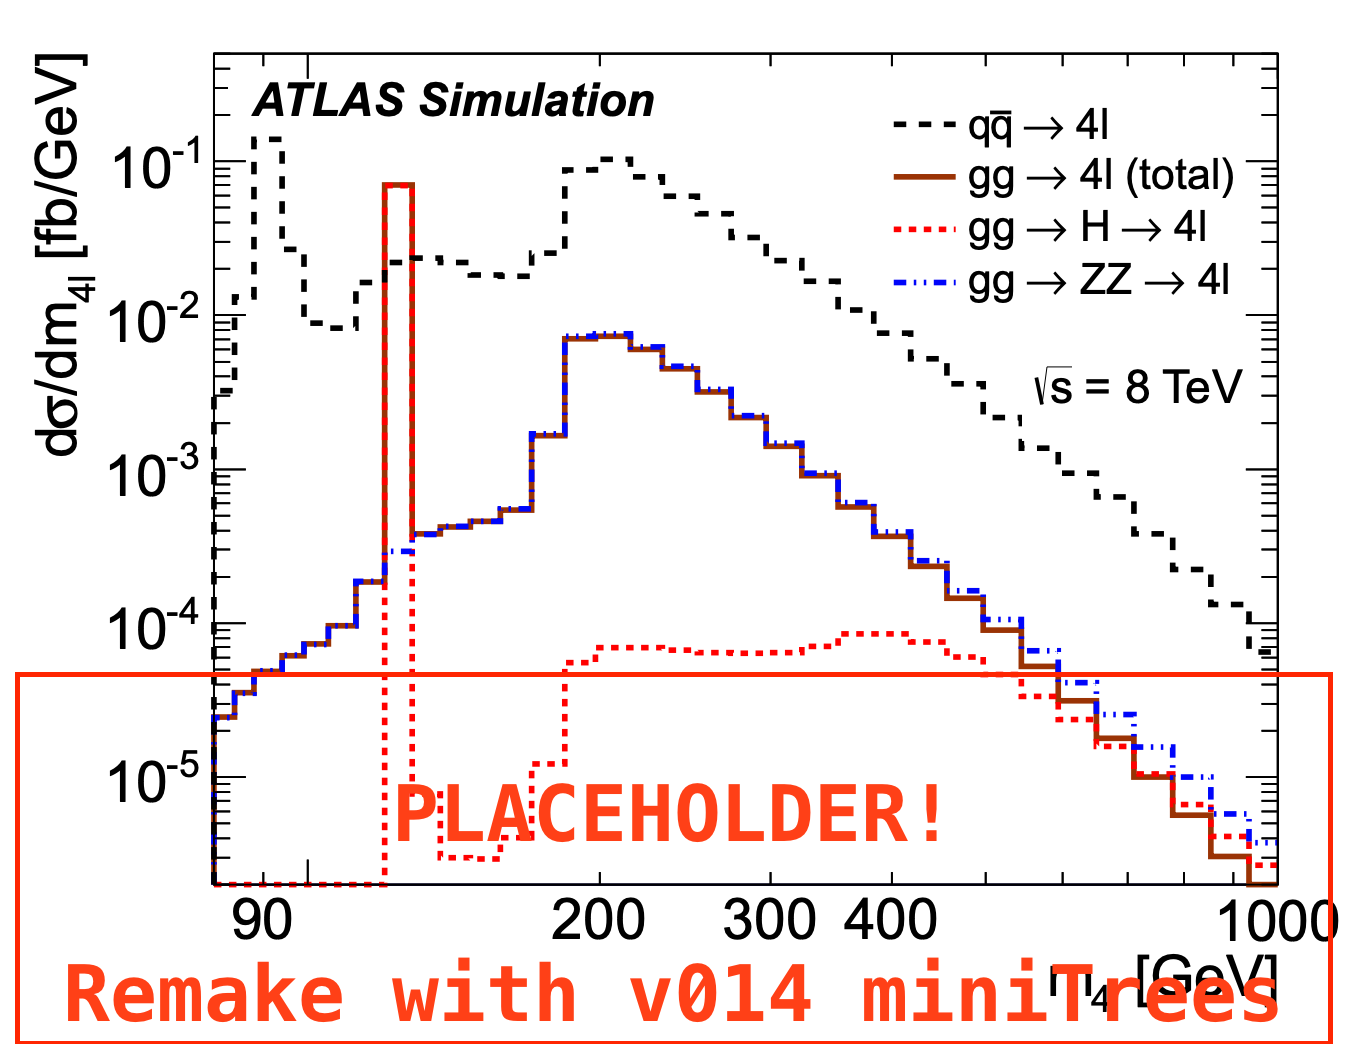
\includegraphics[width=0.5\textwidth]{Figures/m4l/m4lbreakdown.png}
    \caption{Breakdown of contributing processes contributing to the \mFourL distribution.}
    \todo[inline]{Replace and remake with our miniTrees.}
    \label{fig:m4lbreakdown}
\end{figure}

\begin{figure}
\centering
\begin{subfigure}{.24\textwidth}
  \centering
  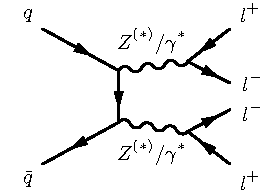
\includegraphics[width=.23\textwidth]{Figures/FeynGraphs/qqZZ4l.pdf}
  \caption{\qqZZ}
  \label{fig:m4lfeynman:qqZZ}
\end{subfigure}%
\begin{subfigure}{.24\textwidth}
  \centering
  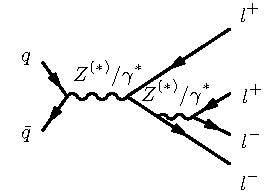
\includegraphics[width=.23\textwidth]{Figures/FeynGraphs/qqZZ4lrad.pdf}
  \caption{A subfigure}
  \label{fig:m4lfeynman:singleZ}
\end{subfigure}
\begin{subfigure}{.24\textwidth}
  \centering
  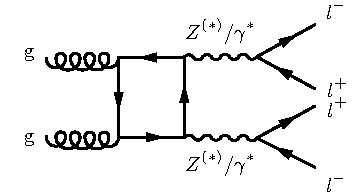
\includegraphics[width=.23\textwidth]{Figures/FeynGraphs/ggZZ4lbox.pdf}
  \caption{A subfigure}
  \label{fig:m4lfeynman:ggZZ}
\end{subfigure}
\begin{subfigure}{.24\textwidth}
  \centering
  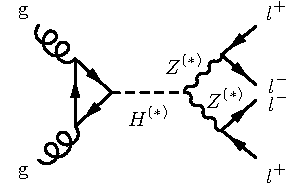
\includegraphics[width=.23\textwidth]{Figures/FeynGraphs/ggZZ4lhiggs.pdf}
  \caption{A subfigure}
  \label{fig:m4lfeynman:ggHZZ}
\end{subfigure}
\caption{Feynman diagrams for quark- and gluon-induced \ZZ production. The processes shown are the main contributors.}
\label{fig:m4lfeynman}
\end{figure}

% this channel provides a clean leptonic final state resulting in a small instrumental background, where one or more of the reconstructed lepton candidates originate from the misidentification of jet fragments or from nonprompt leptons.

%% Signal definition and event selection
\section{Signal and fiducial region definition}
\label{sec:signaldef}

The motivation behind this analysis is to make a measurement as inclusive and as model-independent as possible. Any process leading to a final state of four lepton - made up of two same flavour opposite sign electron or muon pairs - is considered to be part of the signal. Electrons or muons originating from fully leptonic decays of taus are counted towards the signal. 

The fiducial region definition follows closely the acceptance of the detector. Furthermore, by loosening the mass cuts, there is higher event acceptance especially in the low mass regions. Preliminary studies were conducted to investigate the impact of loosening and simplifying the dilepton lower mass cut to \unit{5}{\GeV} and removing the upper mass cut, for example, as opposed to the varying higher cuts in the previous round of the analysis. Unsurprisingly, these result in a higher event yield in both the low and high mass tails of the \mFourL distribution. 

The final state is defined solely in terms of final state particles as opposed to targeting a specific process. Beyond the requirement of two same flavour opposite sign lepton pairs, the measurement is inclusive to additional particles such as additional leptons, jets, and invisible particles. Previous irreducible backgrounds (\VVV, \ttZ) are now considered as part of the signal since they produce four or more prompt leptons.

\missingfigure{Emily plots for loosening mass cuts}

\subsection{Lepton definitions}

For particle physicists, a prompt lepton simply means the lepton did not originate from a hadron. Prompt leptons are further classified into three categories depending on their association with emitted photons. These three categories are:
\begin{itemize}
    \item Born leptons: leptons prior to QED Final State Radiation (FSR);
    \item Bare leptons: leptons after QED FSR;
    \item Dressed leptons: leptons after QED FSR, that then have the four momenta of nearby radiated photons added to it. 
\end{itemize}
The ATLAS detector makes lepton measurements after QED FSR has occurred. It is for this reason that born leptons are not the best choice. It is more realistic to perform measurements involving only final state particles, and objects constructed from final state particles, such as dressed leptons \cite{Kar:ab1be6}. 

\subsubsection{Dressed electrons and bare muons}

In this analysis, a choice of dressing electrons but leaving muons bare was made to closer mimic what is seen by the detector. 

%% Truth isolation
When selecting leptons in the data, there is a complex isolation criteria applied \todo[]{What is this isolation criteria?}. An emulation of this reconstruction-level criteria is included in the fiducial region definition. Although the particle-level application is a simplification, it nevertheless returns a result that is closer to what is actually measured. The particle-level truth isolation criteria requires the sum of the transverse momentum of all charged particles inside a $\Delta R  = 0.3$ cone of the lepton, divided by transverse momentum of the lepton itself, to be less than 0.16. If any other selected leptons are within the cone, their
momenta is not included. 
$$\dfrac{\pt(\Delta R  = 0.3)}{\pt(\text{lepton})}<0.16$$
\subsection{Fiducial region}

\begin{table}[bp]
  \begin{tabular}{lllll}
        & Lepton requirements \\
        \midrule
        Electrons & Dressed lepton definition\\
                & \pt > \unit{5}{\GeV}\\
                & $|\eta| < 2.47$\\
        Muons & Bare lepton definition\\
            & \pt > \unit{7}{\GeV}\\
            & $|\eta| < 2.7$\\
        \bottomrule
        \toprule
        & Event requirements \\
        \midrule
            Four-lepton signature & At least 4 leptons, with 2 Same-Flavour, Opposite-Sign pairs \\
               Lepton kinematics   &   $\pt > 20 / 10$~\GeV{} for
                                     leading two leptons \\ [0.3cm]
              Lepton separation               &   $\Delta R_{ij} > 0.05$ for any leptons \\
              $J/\psi$-Veto &    $  m_{ij} > 5$~\GeV for all SFOS pairs \\
              Truth isolation & ptcone30/\pt < 0.16 \\
  \end{tabular}
  \caption{Fiducial region definition.}
  \label{tab:fidregion}
\end{table}

\missingfigure[]{Dressed electrons, bare muons plot}

\subsection*{Lepton pairing and quadruplet formation} 
\todo[inline]{Reword this whole subsection!!}
Events satisfying the requirements described above enter the fiducial region of the measurement. 
In order to define observables, a unique set of exactly four leptons per event is chosen: 
\begin{itemize}
\item First, the SFOS lepton pair with an invariant mass closest to the Z boson mass is selected as the primary pair in the event. 
\item The remaining SFOS lepton pair closest to the Z boson mass is then referred to as the secondary pair, and completes the quadruplet. 
\end{itemize}
In this way, only one quadruplet is defined even in events containing more than four leptons.
This selection strategy is chosen since it prefers to form pairs that correspond to on-shell Z bosons for the dominant $ZZ$ pair production process, making the pair-level observables based on this definition comparable to such obtained in dedicated $ZZ$ production measurements. This is explored further in Appendix~\ref{app:pairing}. 
The pair and quadruplet formation does not have any impact on the event selection outcome. 

%% Theoretical predictions 
\section{Data andMonte Carlo predictions}
\label{sec:montecarlo}

Theoretical predictions from Monte Carlo simulations

\section{Measured observables}

The star observable of the analysis is none other than the four lepton invariant mass, \mFourL. It has been measured previously by both the \ATLAS and the \CMS experiment \todo{missing citation} \cite{}. As with the previous round of the analysis, the \mFourL distribution is also measured double-differentially, in slices of the transverse momentum of the four lepton system, the absolute rapidity of the four lepton system, and the flavour channel of the four lepton system. 

New to this round of the analysis is the division of the four lepton invariant mass spectrum into four separate regions, each dominated by a different process. From \unit{60}{\GeV}-\unit{100}{\GeV} resonant single \Z production reigns, similarly the \unit{120}{\GeV}-\unit{130}{\GeV} region is dominated by Higgs production, and the high mass region from \unit{180}{\GeV}-\unit{2000}{\GeV} by on-shell \ZZ production. Lastly to fill the gaps between  \unit{20}{\GeV}-\unit{60}{\GeV}, \unit{100}{\GeV}-\unit{120}{\GeV}, and \unit{130}{\GeV}-\unit{180}{\GeV} is the off-shell \ZZ region. This is summarised in Table \ref{tab:m4lregions}. The following variables are measured double differentially in these four regions:

\begin{itemize}
    \item Cosine of angle $\theta^{*}$, where $\theta^{*}$ is the angle between the \todo{definitely check this} lepton in the rest frame and the \Z boson in the lab frame. This angle is sensitive to the polarisation of the decaying boson.
    \item The difference in rapidity between the lepton pairs
    \item The difference in azimuthal angle between the lepton pairs, and between leading leptons
    \item The invariant mass of the lepton pairs
    \item The transverse momentum of the lepton pairs
\end{itemize}

\begin{table}[bp]
  \begin{tabular}{lllll}
        Region & \mFourL interval(s) \\
        \midrule
        \ZFourL & \unit{60}{\GeV} < \mFourL < \unit{100}{\GeV} \\
        \HFourL & \unit{120}{\GeV} < \mFourL < \unit{130}{\GeV} \\
        On-shell \ZZ & \unit{180}{\GeV} < \mFourL < \unit{2000}{\GeV} \\
        Off-shell \ZZ & \unit{20}{\GeV} < \mFourL < \unit{60}{\GeV}, \unit{100}{\GeV} < \mFourL < \unit{120}{\GeV}, \\
          & and \unit{130}{\GeV} < \mFourL < \unit{180}{\GeV}\\
  \end{tabular}
  \caption{The four \mFourL regions dominated by the single \Z, Higgs, on-shell and off-shell \ZZ processes.}
  \label{tab:m4lregions}
\end{table}

\section{Event reconstruction and selection}
\todo[inline]{Change from here on}


To define observables in the events selected this way, a quadruplet of baseline leptons is selected. 
This must consist of two same-flavour opposite-sign(SFOS) pairs, and the combination with lepton pair invariant masses closest to that of the $Z$ boson mass is selected. The lepton pair with invariant mass closest to the $Z$ mass is designated the leading pair, and the sub-leading lepton pair with mass closest to the $Z$ boson mass is then selected from the remaining possibilities.

Finally, the four leptons forming the quadruplet are further categorised, as detailed in Table~\ref{tab:signalLeptons}. 
Baseline leptons are designated as ``signal'' leptons if they satisfy a range of requirements designed to suppress leptons not originating from the hard scatter as well as misidentifications.
They are required to be isolated, using the FixedCutPflowLoose working point, which is designed to be robust to pile-up and was found to have the best efficiency over the full invariant mass range, as can be seen in Appendix~\ref{app:iso}. In order to remain sensitive to scenarios where the leptons are highly collimated, i.e. if they are produced by a very boosted particle, contributions from close-by leptons are subtracted from the isolation variables using the 'IsolationCloseByCorrectionTool' CP tool supported by the identification and fake forum before the cuts are applied. In addition, both electrons and muons are required to pass track-to-vertex criteria, with selections on the impact parameter and interaction point. Finally, electrons are required to satisfy the LooseBlayer identification criterion, which adds a requirement on hits in the innermost pixel layer to the Loose working point used to define baseline electrons. 
\todo[inline]{Change from here up}

 \begin{table}[ht]
    \centering
        \begin{tabular}{l | l c }
            Category & Requirement \\
            \hline
            \hline
            Kinematics & Muons : & $\pt > 5$~\GeV{} \\
                       &         &  If CaloTag: $> $15~\GeV \\
                       &         &   $|\eta| < 2.7$  \\[0.2cm]
                       & Electrons: & $\pt > 7$~\GeV \\
                       &            & $|\eta| < 2.47$  \\ 
            \hline
            Vertex association 
                       & Both : & $|z_{0}\dot \sin{\theta}| <$0.5~mm \\
            \hline Identification: 
                       & Muons: & Loose ID  \\ 
                       & Electrons: & LooseLH ID  \\
            \hline
            Overlap removal: Lepton-favoured \\ 
        \end{tabular}
    \caption{Definition of the baseline lepton selection.\label{tab:baselineLeptons}}
\end{table}  
          
\begin{table}[ht]
    \centering
        \begin{tabular}{l  c }
            Input objects &  Baseline electrons and muons that are part of the quadruplet \\ 
            \hline
            Isolation  &   FixedCutPflowLoose working point\\ %add more detail here/elsewhere
                       &   \textit{Contribution from all other baseline leptons is subtracted} \\
            \hline    
            Cosmic muon veto & Muons: $|d_{0}| < $1~mm\\
            \hline
            Impact Parameter &  Muons: $d_{0}/\sigma_{d_{0}} < $3 \\
                             &  Electrons: $d_{0}/\sigma_{d_{0}} < $5 \\
            \hline
            Stricter Electron ID &  Electrons: LooseBLayerLH ID \\
        \end{tabular}
        \caption{Definition of the signal lepton selection.\label{tab:signalLeptons}}
\end{table}


\begin{table}[ht]
    \centering
        \begin{tabular}{l | c }
            Category & Requirement \\
            \hline
            Event Preselection & Fire at least one lepton \\
                                & trigger \\
                               & $\geq$1 vertex with 2 or more tracks \\[0.2cm]
            \hline
               Four-lepton signature & At least 4 leptons ($e,\mu$)    \\ 
               Lepton kinematics   &   $\pt > 20 / 10$~\GeV{} for
                                     leading two leptons \\[0.2cm]
               Lepton separation               &   $\Delta R_{ij} > 0.05$ for any two leptons \\
              $J/\psi$-Veto &    $  m_{ij} > 5$~\GeV for all SFOS pairs \\
            \hline 
               Trigger matching   & Baseline leptons matched to at least one lepton trigger \\[0.2cm] 
            \hline
              Quadruplet & At least one quadruplet with 2 Same-Flavour, \\
              formation & Opposite-Sign (SFOS) pairs \\
            \hline
              Quadruplet &  4 signal, 0 non-signal: signal region \\
              categorisation    &  $\leq 3$ signal, $\geq 1$ non-signal: background control region \\
        \end{tabular}
        \caption{Definition of the reconstruction-level selection.\label{tab:eventsel}}
\end{table}

\section{Background estimation}
\label{sec:background}

\subsection{Defining leptons}

The four lepton channel is quite the golden channel, as it has a very clean signature with minimal background. In fact, the single dominant background in this analysis is when one or more of the reconstructed leptons in the quadruplet are not real leptons; rather they are misidentified objects in the detector mimicking the same signature \cite{varnes2016poisson}. These "leptons" are non-prompt, and can be referred to as a fake lepton, whereas a lepton produced from the hard scatter is a prompt, real lepton. One source of fake leptons is from hadron decays. In the case of the electron, photon conversion and hadronic jets misidentified due to their large and narrow deposit in the electromagnetic calorimeter can also play a role. In this analysis, around three-quarters of the fakes originate from \Pbottom-hadron decays in \Z plus jets and \Ptop\APtop events. 

The size and behaviour of the fake lepton background - also referred to as the reducible background - are usually estimated using data-driven methods because they are not well modelled by simulation \cite{varnes2016poisson}. One such method is the Fake Factor method. This method depends on two sets of lepton criteria: a tight criteria that selects leptons which make it into the signal region, and a loose criteria that is similar but less restrictive. The leptons selected by the latter are referred to as baseline leptons, and the baseline leptons that additionally pass the tight criteria are the signal leptons. The rest of this section will also touch on baseline-not-signal leptons; these are leptons that pass the "baseline" loose selection, but do not make the "signal" tight selection. 

\subsection{Fake Factor method}

The Fake Factor method relies on the calculation of a fake efficiency, $f$, which is the fraction of fake baseline leptons pass the tight selection criteria and become signal leptons. Because fake leptons not well modelled in simulation, the fake efficiency is calculated in data, in an alternative region of phase space that is enriched with fake leptons. 

Using the Fake Factor $F$, the number of baseline leptons, and the number of real baseline leptons, the number of fake signal leptons can be calculated. Note that the FF method assumes good modelling in the real component of the simulation since $N^{\text{baseline}}_{\text{real}}$ is taken from MC.

$$N_{\text{fake}}^{\text{signal}} = F(N^{\text{baseline}}-N^{\text{baseline}}_{\text{real}})$$

%% Smoothing

Smoothing on the raw output of the reducible background estimate is performed. The raw output, due to low statistics in certain bins, have pronounced, jagged features that resemble resonances. Of course, resonant peaks should not exist. The smoothing procedure is therefore used to obtain a more even shape, minimising the impact of any outlier bins that had a large Fake Factor weight. In order to smooth the distribution, an intermediate, finer binning is assigned to each observable and the background estimate is run. The fine-binned intermediate background distribution is smoothed with Friedman's super smoother. Lastly, the final background estimate is obtained by integrating over the smoothed distribution using the coarser, original binning. A visualisation of the process is shown in Figure \ref{fig:backgroundsmoothing}.

\missingfigure{background smoothing}

\section{Systematic uncertainties}
\label{sec:sysuncert}

\subsection{Experimental uncertainties}

Lepton (electron an muon) identification, reconstruction and isolation efficiencies.
Trigger efficiency.
Lepton momentum and scale uncertainties.
Pile-up rescaling.
Luminosity.

\subsection{Theoretical uncertainties}
QCD scale uncertainties.
PDF uncertainties.
Parton shower.
EW NLO reweighting.

%% Unfolding and respective studies
\section{Correcting for detector effects}
\label{sec:unfolding}

When an observable is measured by a particle physics experiment, it is important to note that the measured distribution, (i.e. what the particle detector sees) is not what truly occurs at the particle-level. Rather, it is a convolution of the underlying physics process with the effects of the detector. The \ATLAS detector, although an astonishing feat of technology, is still subject to resolution, acceptance, and efficiency limitations. The data at the detector level is smeared and includes the effects of these limitations. For an inclusive measurement such as the four-lepton invariant mass distribution, it is often desirable to correct for these detector effects and present the data at the particle-level. In doing so, the measurement may be directly compared to theoretical predictions, as well as particle-level results from other experiments, in the years to come. In high energy physics, the term coined for this correction procedure is unfolding.

When Unfolding Makes Sense
4
1. Results from experiment A and B with different response function are to be
compared
2. It is too complicated to publish the response function of the detector along
with the data
Detector response might be very complex, e.g., time dependent
Sometimes computer code reflecting the response would have to be published
Danger that future users don't use the filter correctly

\subsection{Unfolding methodology}
\label{subsec:unfmethod}

Unfolding in particle physics can be more generally referred to as a deconvolution. The generic problem statement of deconvolution is to derive a relationship between the true distribution $T(x)$ and the recorded distribution $D(y)$. The two are related by a smearing function $R(x,y)$, which encompasses the instrumentation effects in making the measurement. 
\begin{equation} \label{eq:unfintegral}
    T(x)=\int S(x,y)D(y)dy
\end{equation}
Due to the discretized nature of histograms, the unfolding problem can be stated as a matrix equation:
\begin{equation} \label{eq:unfmatrix}
    x_i=S_{ij}y_j
\end{equation}
where $R$ represents the a smearing matrix of sorts, \todo{add more}$T$ is the true histogram at particle-level, and $D$ is the reconstructed histogram at detector-level. 

For the four-lepton invariant mass analysis, an iterative unfolding method motivated by Bayesian statistics, popularised by Giulio D’Agostini, is chosen. The method iteratively applies the three inputs described above to the measured distributions while using the particle-level SM prediction as a prior.

\subsubsection{An iterative Bayesian approach to unfolding}
\label{ssec:bayesianunfolding}
Let there be a set of causes $C_i$, that can produce one effect $E$. 
\begin{equation}
    P(C_i|E)=\dfrac{P(E|C_i)\cdot P(C_i)}{\Sigma_{k=1}P(E|C_k)\cdot P(C_k)}
\end{equation}

\begin{itemize}
    \item $P(C_i|E)$: given the effect, ithe conditional probability that it was produced from the $i$-th cause.
    \item $P(E|C_i)$: for the $i$-th cause, the conditional probability that the effect is produced.
    \item $P(C_i)$ is the initial probability of the $i$-th cause.
\end{itemize}
If there are multiple possible effects for the causes, then the formula can be generalized to be:
\begin{equation}
    P(C_i|E_j)=\dfrac{P(E_j|C_i)\cdot P(C_i)}{\sum_{k=1}P(E_j|C_k)\cdot P(C_k)}
\end{equation}
The number of expected events for each cause $C_i$ can be obtained by multiplying the number of observations made for effect $j$ with the probability it had been due to cause $i$, and summing over all effects:
\begin{equation} \label{eq:numcause}
    N(C_i)=\sum_jN(E_j)\cdot P(C_i|E_j).
\end{equation}
Here a parallel can be drawn back to equation \ref{eq:unfmatrix}, where $N(C)={N(C_1),N(C_2),...,N(C_n)}$ represents the number of events in the $n$ bins of the true histogram $x_i$, and $P(C_i|E_j)$ corresponds to $R$. Combining these equations, the procedure for estimating the true histogram can be written as:
\begin{equation}
    x_i=\sum_{j=1}^n\dfrac{R_{ij}\cdot P(x_i)}{\sum_{k=1}^nR_{kj}\cdot P(x_k)}y_j.
\end{equation}
Here the matrix defined as $R_{ij}$ is the response matrix. The denominator in the equation is a normalisation factor using the y-projection of the matrix. $P(x_i)$ is the prior, which is updated in each iteration with the unfolded true distribution $x_i$, also known as the posterior.
\todo[inline]{Perhaps mention other unfolding methods and justify choice of this one?}

\subsubsection{Unfolding inputs}

In this analysis the variables of interest are presented as histograms with a finite number of bins. In order to bring these distributions from reconstruction-level to particle-level, there are a number of correction factors to consider:

\begin{itemize}
    \item Fiducial fraction: this is a one-dimensional correction that accounts for events which do not enter into the fiducial region, but pass the detector-level selection nonetheless. These occur due to the finite resolution in the measurement the variables used to select events. The fiducial fraction is defined as the ratio of events that pass both fiducial and detector-level selection to events that pass detector-level selection only.
    \item Reconstruction efficiency: this accounts for the acceptance and efficiency of the detector in reconstructing an event. Of all the events that pass the fiducial selection, only a fraction will be successfully reconstructed and visible to the detector. Formally the reconstruction efficiency is also a one-dimensional correction; defined as the ratio of events which pass both the fiducial and detector-level selection to events that pass fiducial-level selection only.
    \item Migration matrix: each bin in the histogram of the measured observable represents a sub-range of observable values. Sometimes the detector may smear the observable's value high or low enough such that it gets filled to different bins in particle-level and detector-level. These are referred to as bin-to-bin migrations, and is corrected for by the migration matrix. This is constructed as a two-dimensional matrix using events which pass both fiducial and detector-level selection, with the value at particle-level on one axis and the value at detector-level on the other. The matrix, $M_{ij}$, represents the probability that an event which falls into bin $i$ at particle level will fall into bin $j$ when reconstructed at the detector-level. 
\end{itemize}

\subsubsection{Number of Bayesian iterations}

When using the iterative Bayesian method to unfold, the number iterations performed is a key parameter and must be optimised. The method, which uses the nominal MC distribution as an initial prior, results in a bias towards the original shape of the nominal prediction. A way to minimise this effect is to use the obtained unfolded distribution from the previous iteration as the prior for the subsequent unfolding iteration. The more iterations there are, the less dependence there is on the prior, and therefore the smaller the bias. A side effect, however, is that increasing the number of iterations also increases the statistical uncertainty. Fluctuations caused by limited statistics become amplified by the feedback in the algorithm. These effects are thoroughly studied in order to strike a balance between minimising the bias at the cost of increasing the statistical uncertainties.

One thousand toy distributions are generated using the detector-level Standard Model prediction where the value of each bin is randomly drawn from a Gaussian distribution. Each toy is unfolded following the procedure outlined in section \ref{ssec:bayesianunfolding}, where the nominal SM predictions are used to construct the response matrix and for the prior. The bias, written as
\begin{equation} \label{eq:unfbias}
    \text{Bias}_i=\dfrac{\sum_{j=1}^nM_{ij}\cdot x_j-y_i\cdot f_i}{y_i\cdot f_i},
\end{equation}
measures the difference between the product of the migration matrix and the unfolding output, and the product of the detector-level toy and the fiducial fraction. It is an assessment of the strength of the pull that the shape of the SM prior has on the unfolded toy result \todo{Read more about regularisation}. Additional, a statistical uncertainty from the unfolding procedure for each individual toy in each bin is quoted. Next, the bias significance\change{italics?} per bin is defined as the quotient of the bias and the statistical uncertainty. After sampling over all toys, the root-mean-square of the bias significance in each bin is calculated. Through the rms bias significance, the size of the bias in comparison to that of the statistical uncertainty is quantified and used as a criterion in determining the number of iterations. The requirement is to use the minimum the number of iterations needed for a bias significant lower than 0.5.

\missingfigure{Optimisation of number of unfolding iterations}

Figure \ref{fig:unfopt} shows the bias, the statistical uncertainty, and the rms bias significance for the inclusive \mFourL distribution. Here the minimum number of iterations for which the criterion is met is three. For the majority of the other measured distributions, three iterations of the unfolding are also found to be optimal. Two iterations are found to be sufficient for the following observables: \mZOne-\mFourL, \dPhill-\mFourL, and \dYPairs-\mFourL.

\subsection{Binning optimisation}
\label{subsec:binningopt}

The binnings of the measured distributions were optimised based on two factors: the number of events and the purity of each bin. Here the purity refers to the diagonal of the migration matrix normalised along truth, thus representing the fraction of truth events that end up in the same reconstructed event bin. There were a few iterations of the binning that were run with varying criteria, summarised in table \ref{tab:BinningVersions}.

The first iteration of the binnings were run with the nominal criteria. Here, depending on the number of events in the bin, the purity requirement varies. Bins with lower statistics have a high purity requirement to reduce bin-to-bin migrations. The minimum number of events required for each bin is 14. Between 14 and 20 events, the purity was required to be at least 80\%. Between 20 and 25 events the purity must be 70\% or higher. Finally for the higher statistics bins with more than 25 events the purity cut was 60\%. 

The binning algorithm is as follows. For the full \mFourL differential mass distribution from \unit{20}{\Gev} - \unit{2000}{\GeV}, the distribution was first split into very fine steps of \unit{1}{\GeV} bins from \unit{20}{\Gev}-\unit{450}{\GeV}. From \unit{450}{\Gev}-\unit{2000}{\GeV} wider steps of \unit{5}{\GeV} bins were used. Due to the fine nature of the bin widths, this initial binning failed to meet any of the binning criteria. Next, the binning algorithm starts from the low mass end and starts to merge adjacent bins together if the criteria were not met. For example, if bin number 1 [20,21] has > 10 events, the algorithm merges bin number 1 with the next bin. The new bin number 1 is now [20,22]. Once again, if this bin has > 10 events, it will merge again and become [20,23], and so on and so forth until 10 events has been reached. Of course the purity must also pass the required percentage for the number of events in the bin, otherwise further bin merging occurs.  

Next we have the \mFourL distributions in double differential slices of \ptFourL, \yFourL, and flavour channel. For these distributions, the fine binning was defined as the the binning of the full \mFourL differential mass distribution, i.e. the output of the algorithm described in the previous paragraph. Bins were once again checked for number events and purity, and merged as needed. This was implemented so that all \mFourL in each of the  \ptFourL, \yFourL, and flavour slices would have bin edges that match with the inclusive distribution. 

For the distributions measured double differentially in the four \mFourL regions corresponding to \Z, \Higgs, On-shell \ZZ, and Off-shell \ZZ, the same procedure was followed for binning optimisation. Each distribution had a fine binning defined, and the bins were merged from left to right of the x-axis until the criteria were met. 

\begin{table}[bp]
  \begin{tabular}{lllll}
                & Nominal              & High statistics             \\
    \midrule
                                & 14 (purity > 0.8) &   \\
     Minimum number of events & 20 (purity > 0.7) & 100    \\
                                &25 (purity > 0.6) &    \\
  \end{tabular}
  \caption{Three different versions of binning with varying criteria.}
  \label{tab:BinningVersions}
\end{table}

\subsection{Pre-unfolding weights}
\label{subsec:preuf}

When correcting the data for detector effects, one of the things to take into account is the efficiency correction. Recall from section \ref{subsec:unfmethod} that the efficiency correction is the fraction of reconstructed events that also pass the fiducial selection cuts. A significant contribution to this is the efficiency correction is efficiency in identifying, reconstructing, isolating, and track-to-vertex-association of (TTVA) leptons. These are dependent on lepton kinematics and calculated from Monte Carlo simulation, therefore they may not be accurate if the data differs from the prediction. To correct for this effect, the lepton efficiencies are measured as a function of the lepton transverse momentum (\pt) and pseudorapidity ($\eta$), and the inverse of this is applied as a per-lepton weight in the data. The term coined for this weight is the pre-unfolding weight, and as the name suggests it is applied prior to the unfolding procedure detailed in \ref{subsec:unfmethod}. 

\missingfigure{Detector yield with and without pre-UF, and efficiency corrections}

Figure \ref{fig:preUF} shows the detector yield from simulation with and without the application of the pre-unfolding weights, compared to the particle yield. It is readily apparent that the detector yield comes much closer to the particle yield when pre-unfolding weights are applied. In some cases, the detector yield surpasses the particle yield around the resonance peaks. This is attributed to bin migrations, and has negligible effects on the final unfolded result. Also shown is the efficiency correction with and without the pre-unfolding weights. In general, a significant increase in efficiency throughout the whole \mFourL spectrum, ranging from 10\% at low mass, up to 25\% at high mass. The conclusion drawn from these plots is that a large portion of the event inefficiency can be accounted for using per-lepton corrections, bringing the reconstructed and particle level yield closer to one another, and minimising the correction needed when unfolding.

\subsection{Closure tests}
\label{sec:closuretests}
\subsubsection{Monte Carlo closure tests}

As detailed in section \ref{subsec:unfmethod}, the unfolding procedure uses a response matrix that has been derived from Standard Model Monte Carlo predictions. A simple test that can be performed to check the validity of the unfolding method is to use the same SM MC prediction at reconstruction level as pseudodata, unfold it, and compare it to the truth level prediction. This is a self-consistency check, and should yield the trivial result that the unfolded pseudodata be identical to the truth distribution. This is the full MC closure test, and acts as a sanity check for the unfolding procedure.

Another similar validation, the half-half MC closure test, is also performed. This time, the SM samples are divided in two sets A and B based on whether their tagged event number is odd or even. Set A is used to construct the fiducial fraction, reconstruction efficiency, and migration matrix, while set B is used as pseudodata and unfolded with the inputs from the set A. The unfolded distribution of the set B is then compared to the true distribution of the set B.

\missingfigure{Show full MC closure test}
\missingfigure{Show half-half MC closure test}

\subsubsection{Data-driven closure tests}
\todo[inline]{TO-DO!}

\subsection{Injection studies}
\label{subsec:injection}

Section \ref{sec:closuretests} demonstrates that the unfolding procedure has closure when unfolding pseudodata that agree with the Standard Model. Since the SM predictions themselves were used to derive the corrections and matrix used for unfolding, this is the expected case. The shape of real data is unknown, however, and may be different than the Standard Model prediction. Should the \mFourL spectrum be host to contributions that differ from the SM prediction, it is necessary to check that the unfolding procedure is nonetheless able to provide an accurate and unbiased particle-level result. In order to do this a number of injection tests were performed. The first step is to take the nominal SM prediction, and inject some amount of BSM signal into it. The reconstruction level yield of this modified sample is used as pseudodata. It is run through the standard unfolding workflow in entirety, and compared to the particle level yield of the modified sample. Conceptually, this procedure is very similar to that of the Monte Carlo closure tests. 

A number of modifications were made to the nominal SM prediction, one set had the addition of a gluon-gluon fusion produced heavy Higgs boson with a mass of 300, 800, or \unit{1400}{\GeV} with either a narrow width or a width 15\% of its mass, and another set where the heavy Higgs was produced via vector-boson fusion. The \ggZZ process was also modified to have a larger event weight with respect to the SM prediction. These are described in full in Table \ref{tab:injectionsamples}. 

\begin{table}
    \begin{tabular}{lll}
                            & Injection samples & \\
        \midrule \\
                            &               & 300 GeV \\
         Gluon-gluon fusion &  Narrow width & 800 GeV\\
                            &               & 1400 GeV \\
                            &               & 300 GeV \\
                            & 15\% width    & 800 GeV \\
                            &               & 1400 GeV \\
         \midrule \\
                                & & 300 GeV \\
         Vector-boson fusion    & & 800 GeV \\
                                & & 1400 GeV \\
         \midrule \\
         \ggZZ enhancement & \\
    \end{tabular}
  \caption{Modifications made to the nominal SM prediction for injection studies.}
  \label{tab:injectionsamples}
\end{table}

For each of the variations listed in Table \ref{tab:injectionsamples}, a range of cross-sections were injected and then unfolded with and without application of the pre-unfolding weights. In order to carve a more realistic scenario, one of the injected cross-sections for the heavy Higgs samples was set to be just within the two-sigma band of the data uncertainty. This was done by increasing the injected cross-section and calculating the $p$-value between the BSM prediction and the data until a $p$-value smaller than or equal to 0.05 is reached\footnote{This is the $p$-value corresponding to a two-sigma significance.}.

\missingfigure{Injection test plots, show only two sigma ones}

\section{Results}
\label{sec:results}

\section{Interpretations}
\label{sec:interpretations}

\subsection{\ZFourL branching fraction}

\subsection{Limits on B-L model}

\subsection{EFT couplings}

A simple example of an effective field theory is the Fermi theory of beta decay. In this theory postulated in 1933, the neutron decay occurs in a point-like manner to an electron, a proton, and a neutrino. The effective Lagrangian describing this interaction constant $G_{\text{F}}$, the Fermi constant, which is proportional to the ratio of the weak coupling constant to the mass of the $W$ boson. This was only discovered later on, however, and at the time knowing only the Fermi constant was a sufficient way to model the process. The $W$ boson has a mass that is an order of magnitude higher than the typical energy of $\beta$ decays, and has been integrated out in the Fermi theory. This is said to be an effective field theory calculation, which is consistent way to describe a higher-order process so long as the energy scale of the process is small compared to the energy scale of the mediating heavy state \cite{De_Simone_2016}. 

The SMEFT formulism used here is in the Warsaw basis \todo{cite this}, containing fifty-nine independent operators which assume lepton and baryon number conservation. 
